\newpage
\section{Implementazione}
In questa sezione vengono analizzati gli aspetti implementativi del sistema, facendo eventualmente riferimento al codice
sviluppato. Nello specifico, verranno approfonditi solamente gli elementi che non sono stati esplorati a pieno nella
sezione Design di Dettaglio o che si ritengono fondamentali nello sviluppo di un progetto di tipo "game" come quello in
discussione. Per riflettere la suddivisione del lavoro durante il processo di sviluppo, questa sezione presenta una
parte descrittiva per ognuno dei membri del team.

\subsection{Tommaso Mandoloni}
Il mio compito all'interno del progetto, oltre che collaborare con il team per implementare aspetti e funzionalità
comuni di Model, Controller e design, è stato quello di strutturare e implementare le torri di gioco, intese come entità
di base, i loro potenziamenti e infine l'attore che ne incapsula il comportamento. Inoltre mi sono occupato di tutta
la parte di serializzazione e deserializzazione, in modo da poter wrappare gli oggetti in strutture dati salvabili su
file, oltre che nella collaborazione per la creazione di un attore che sfrutti queste funzionalità.

\subsubsection{File Coder}
L'oggetto \texttt{FileCoder} nasce dall'esigenza di poter salvare i dati di gioco su file in modo da poterli
ripristinare per dare all'utente la possibilità di rigiocare le sue partite preferite. In particolare si tratta della
possibilità per l'utente di poter salvare su file le sue mappe preferite in modo da poterle rigiocare. Il
\texttt{FileCoder} quindi lavora principalmente con due tipologie di strutture dati: un file \textit{json}, in cui
vengono indicizzate e salvate le mappe di gioco, e una lista di tracce.

Il suo compito è quello di serializzare e deserializzare il file \textit{json}, tenendolo aggiornato sulle nuove
tracce che l'utente intende salvare. Per supportare la fase implementativa è stata utilizzata la libreria \textit{io.circe}
\cite{circe} che agevola la trasformazione di oggetti in file di tipo json. In particolare sono stati implementati
due \textit{custom codecs}, ossia un \texttt{Encoder} che permette di trasformare una lista di tracce nel rispettivo
oggetto \texttt{Json} che andrà poi salvato su file, mantenendone l'indicizzazione e la sequenza di coordinate delle
celle utilizzate per individuare la traccia di gioco, e un \texttt{Decoder} che svolge l'operazione contraria,
prendendo in input un oggetto Json e trasformandolo nella rispettiva lista di tracce, in modo da poterla modificare o
aggiornare durante la fase di gioco. Per realizzare entrambe le funzionalità di codifica, si è scelto di implementare
le operazioni all'interno di oggetti impliciti in modo che fosse sufficiente richiamare la codifica direttamente sul
tipo di file interessato: in questo modo infatti per trasformare una lista di tracce in un oggetto json, sarà
sufficiente richiamare il metodo \texttt{.asJson} direttamente su una \texttt{List[Track]}, mentre viceversa per
ritornare una lista di tracce da un oggetto json basterà invocare direttamente sull'oggetto il metodo
\texttt{.as[List[Track]]}.

\begin{lstlisting}[language=Scala, caption=Impliciti per le operazioni di codifica, label=code:coder]
implicit val trackEncoder: Encoder[List[Track]] =
    (list: List[Track]) => {
    var objects: List[Json] = List()

    for (i <- list.indices)
      objects = objects.appended(
        Json.obj(
          ("id", Json.fromString(i.toString)),
          (
            "cells",
            Json.fromValues(
              list(i).cells
              .map(cell =>
                Json.fromString(
                    "c(" + cell.x + ", " + cell.y + ")")
              )
            )
          )
        )
      )
    Json.obj(("tracks", Json.fromValues(objects)))
}

implicit val trackDecoder: Decoder[List[Track]] =
    (c: HCursor) => {
    val tracks = c
      .downField("tracks")
      .focus
      .flatMap(_.asArray)
      .getOrElse(Vector.empty)
      .flatMap(_.hcursor
                .downField("cells")
                .as[List[String]]
                .toOption)
      .map(s => Term.createTerm(
                    s.mkString("[", ", ", "]")))
      .map(trackFromTerm)
      .toList
      .map(Track(_))

    Right(tracks)
}
\end{lstlisting}

Le effettive operazioni di salvataggio su file e caricamento da esso, sono state implementate tramite
\textit{for-comprehension} sfruttando la libreria \textit{cats.effects.IO} \cite{cats-effects}, grazie alla quale è stato possibile
definire una sequenza di operazioni da eseguire incapsulandone i side effects, garantendone l'esecuzione in un
ambiente safe dal momento che si parla di scrittura e lettura su file esterni. In questo modo si riesce a mantenere
una struttura di codice molto pulita e intuitiva rispettando il KISS principle e sfruttando a pieno la programmazione
funzionale.

Compito estremamente importante del \texttt{FileCoder} è anche quello di eseguire un corretto setup dell'albero delle
directory di gioco una volta avviato. Infatti dovrà preoccuparsi di controllare se esistono le cartelle che
conterranno i file di gioco, ossia il \textit{json} delle tracce e gli screenshot delle mappe, in modo da non
incorrere in errori durante la fase di scrittura e lettura, e, in caso siano assenti, crearle a run-time. Anche in
questo caso, per rispettare il principio KISS e sfruttare i costrutti funzionali, si è scelto di creare all'interno
di un \texttt{Builder}, una monade appositamente strutturata per facilitare le operazioni di setup. Infatti in questo
modo sarà possibile controllare l'esistenza delle directories di gioco all'interno del file system ed eventualmente
crearle, tutto attraverso poche righe di codice eseguite all'interno di un metodo \texttt{setup} che sfrutta una
sequenza di operazioni eseguite tramite \textit{for-comprehension}.

\begin{lstlisting}[language=Scala, caption=Monade per le operazioni di setup, label=lst:setup]
implicit class FileMonad(path: String) {
  def check: Option[String] =
    if (Files.notExists(Paths.get(path)))
      Some(path)
    else
      None

  def mkdir: Option[file.Path] =
    if (check.isDefined)
      Some(Files.createDirectories(Paths.get(check.get)))
    else
      None

  def touch: Option[file.Path] =
    if (check.isDefined)
      Some(
        Files.write(
          Paths.get(check.get),
          List[Track]().asJson
                       .toString()
                       .getBytes(StandardCharsets.UTF_8)
        )
      )
    else
      None
}
\end{lstlisting}

\subsubsection{Torri}
Le torri, insieme ai pallonicini, sono le entità protagoniste del gioco. Infatti, una volta posizionato nella mappa
di gioco, potranno ruotare per mirare ai palloncini che passano all'interno del loro campo visivo, e sparare un
proiettile specifico verso la loro direzione per poterli scoppiare: pertanto il \texttt{trait Tower} estende
\texttt{Entity}, con l'aggiunta di \textbf{mixin} creati ad-hoc per conferire alla torre la capacità di visione di altre
entità che attraversano il suo campo visivo, e la capacità di sparare un proiettile nella direzione specificata.

Per quanto riguarda la struttura delle torri, come espressamente richiesto dai requisiti, esse devono essere
implementate secondo tre diverse tipologie. Per implentare tale requisito, come prima versione si è pensato di
utilizzare il pattern \textbf{Template Method} in modo da creare una classe astratta che rappresentasse una torre
base, ed estenderne le funzionalità implementando sotto classi specifiche. Questo approccio è stato però abbandonato
a seguito di un'analisi di progettazione più approfondita: infatti si è poi scelto di implementare una
\texttt{BaseTower} come \textbf{case class} che implementasse di default tutte le funzionalità che una torre di gioco
deve possedere. Attraverso questo approccio infatti è stato possibile mantenere una metodologia del tutto funzionale
per quanto riguarda la modifica dei valori delle caratteristiche della torre come la sua rotazione o il raggio del
campo visivo: infatti, al contrario di un approccio orientato agli oggetti dove una volta modificati i campi
richiesti veniva semplicemente aggiornato lo stesso oggetto, in questo caso attraverso l'utilizzo del meotodo
\textit{copy()} ogni volta che una torre deve aggiornare un suo campo, l'intero oggetto viene ricreato con i nuovi
valori. In questo modo anche il codice risulta essere più chiaro e pulito, oltre che più funzionale.

A questo punto, per mantenere la divisione delle torri per le varie tipologie, invece che creare delle sotto classi
per ogni tipo di torre, si è scelto di utilizzare un meccanismo puramente funzionale ossia le \textbf{type class}. Le
type class sono un costrutto tipicamente funzionale che supportano un meccanismo di polimorfismo ad-hoc, in grado
quindi di aggiungere funzionalità vincolate a un tipo di dato specifico ma senza toccare il codice. Infatti la classe
\texttt{BaseTower[B]} è una type class sul tipo di proiettile B che utilizza. Per istanziare quindi le varie
tipologie di torri, è stato adottata una rivisitazione del pattern \textbf{Builder}, specificando dei builder
impliciti che generano automaticamente il tipo di torre corretto passando in input il tipo di proiettile richiesto.

\begin{lstlisting}[label=code:builder, language=Scala, caption=Builder delle tipologie di torre]
object TowerBuilders {
    implicit def genericTowerBuilder[B <: Bullet]: TowerBuilder[B] = BaseTower[B](_)
    implicit val dartTowerBuilder: TowerBuilder[Dart] = BaseTower[Dart](_)
    implicit val iceTowerBuilder: TowerBuilder[IceBall] = BaseTower[IceBall](_)
    implicit val cannonTowerBuilder: TowerBuilder[CannonBall] = BaseTower[CannonBall](_)
  }

  def of[B <: Bullet](bullet: B)(implicit towerBuilder: TowerBuilder[B]): Tower[B] =
    towerBuilder.build(bullet).sight(sightRanges(bullet)).ratio(shotRatios(bullet))
\end{lstlisting}

Seguendo questo approccio e sfruttando le potenzialità delle type class, si riesce a garantire enorme flessibilità ed
estendibilità all'intera strttura delle torri, poiché nel caso venisse aggiunta in futura una nuova tipologia di
proiettile, sarà sufficiente creare lo specifico builder per istanziarne la tipologia di torre associata, senza
doverne implementare una classe specifica.

Al fine di agevolare la creazione delle torri di gioco, è stato creato un appostio DSL che permette di istanziare
tipologie di torri specifiche con pochissime righe di codice e in via del tutto funzionale: ad esempio per istanziare
una torre che lancia freccette, con i suoi valori default, basterà scrivere "Arrow tower spawn".

\begin{lstlisting}[label=code:spawn, language=Scala, caption=Spawning delle tipologie di torre]
def spawn: Tower[Bullet] = tower.bullet match {
      case Dart()        => Towers of Dart()
      case CannonBall(_) => Towers of CannonBall()
      case IceBall(_, _) => Towers of IceBall()
}
\end{lstlisting}

Inoltre ogni torre dispone di una funzionalità di \textit{boosting} aggiuntiva che le permette di incrementare i valori
dei suoi campi durante il gioco, in modo che con l'aumentare dei round e quindi della difficoltà, il giocatore riesca
comunque ad avere un supporto adeguato per vincere i round. Rimane nella strategia del player capire quando e quali
potenziamenti fornire alla torre, al fine di massimizzare il punteggio di gioco. La funzionalità di potenziamento
delle torri è stata implementata come una \textbf{implicit class} proprio sulla classe base della torre seguendo il
principio del \textit{Pimp My Library}, in modo da rendere disponibile il metodo \textit{boost} anche se non fa
parte della sua struttura fisica.

Il comportamento delle entità \texttt{Tower} è incapsulato all'interno di un attore, in modo da rispettare il modello
ad attori sul quale si basa l'intera progettazione e struttura di gioco. Il \texttt{TowerActor} viene istanziato una
volta che il player ha deciso di posizionare una torre all'interno della mappa di gioco, e il suo unico compito è
quello di reagire agli eventi di gioco e comportarsi di conseguenza: infatti entrerà in una fase di
\textit{detecting} dove dovrà verificare se stanno passando dei pallonicini all'interno del campo visivo della torre,
e, in caso il suo rateo di fuoco glielo permetta, sparare un proiettile nella direzione del palloncino individuato.

\begin{figure}[H]
    \centering
    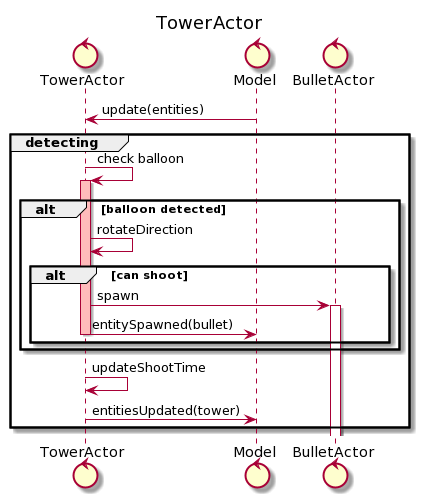
\includegraphics[width=.5\linewidth]{img/tower-actor}
    \caption{Diagramma di sequenza dell'attore delle torri.}
    \label{fig:tower-actor}
\end{figure}

\subsection{Alessandro Marcantoni}
Il mio compito all'interno del progetto è stato quello di realizzare il \texttt{GameLoop}, i palloncini (l'entità base,
i vari "potenziamenti" e infine il rispettivo attore), la gestione dei round (con relativa DSL per la loro creazione e
l'attore che si occupa dello \textit{spawn} dei palloncini) e la suddivisione della logica del model nei tre
\textit{manager}. Ho inoltre collaborato con gli altri membri del team durante la fase di design delle entità.

\subsubsection{Game Loop}
Il \textit{game loop} è il ciclo infinito che si occupa di aggiornare il \texttt{Model} ed ordinare il conseguente
\textit{refresh} della \texttt{View}. Solitamente esso viene implementato mediante un ciclo \texttt{while(true)} ma,
avendo adottato il paradigma ad attori, ciò comporterebbe l'esecuzione di un \textit{handler} bloccante con
conseguente perdita totale di reattività da parte dell'attore \texttt{GameLoop}.

Tale effetto è stato evitato mediante un comportamento che sfrutta un \textit{timer}: l'attore \texttt{GameLoop} invia a
se stesso dei messaggi di tipo \texttt{Tick} distanziati tra loro da un \textit{delay} che dipende dal
\textit{frame rate} scelto per la partita. Alla ricezione di tale messaggio il \texttt{GameLoop} ordina al
\texttt{Model} di aggiornarsi; una volta ottenuta la risposta da quest'ultimo, ordina alla \texttt{View} di renderizzare
la lista di entità provenienti dal \texttt{Model}. Le interazioni appena descritte sono riportate in figura
\ref{fig:sequence-gameloop}.

\begin{figure}[H]
    \centering
    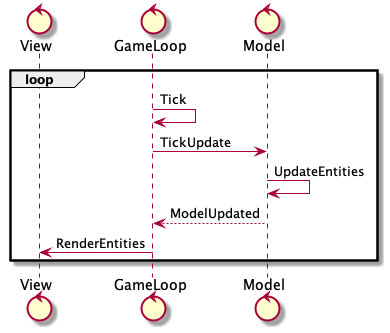
\includegraphics[width=.5\linewidth]{img/sequence-gameloop}
    \caption{Diagramma di sequenza delle interazioni del \texttt{GameLoop}.}
    \label{fig:sequence-gameloop}
\end{figure}

\subsubsection{Palloncini}
I palloncini rappresentano una delle entità fondamentali del gioco. In particolare, essi sono in grado di muoversi
seguendo un percorso e possono essere scoppiati da un proiettile: pertanto, il \texttt{trait Balloon} estende il
\texttt{trait Entity} a cui aggiunge poi le abilità \texttt{TrackFollowing} e \texttt{PoppingAbility} mediante il
meccanismo di \textbf{mixin}.

Per quanto riguarda la loro struttura, i palloncini possono essere \texttt{Simple}, se non ne includono altri al loro
interno, o \texttt{Complex} altrimenti. Tale implementazione permette di rappresentare in modo intuitivo l'effettivo
dominio in quanto, un palloncino complesso, quando scoppiato, deve mostrare il palloncino da lui nascosto.

\begin{figure}[H]
    \centering
    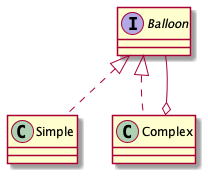
\includegraphics[width=.3\linewidth]{img/class-balloons}
    \caption{Diagramma di classi dei palloncini.}
    \label{fig:class-balloons}
\end{figure}

Tale implementazione rispecchia quella di un \textbf{sum type}: struttura dati tipica della programmazione funzionale.

Degni di nota all'interno del \texttt{trait Balloon} sono i metodi \texttt{change} e \texttt{retrieve}. I palloncini
espongono diversi metodi per accedere o cambiare il valore di proprietà che sono contenute all'interno del
\texttt{Simple}. Dato che l'implementazione di tali metodi sarebbe stata pressoché identica, per meglio aderire al
principio DRY si è deciso di introdurre i suddetti due metodi.
Infine, il metodo \texttt{pop} che elimina un numero di \textit{layer} di \texttt{Complex} pari al danno del proiettile
che colpisce il palloncino. Per fare ciò genera, a partire dal palloncino originale, uno \textit{stream} di questi dove
ognuno rappresenta il palloncino risultante dall'esplosione del precedente. L'utilizzo di \texttt{Option} ha permesso,
attraverso il comportamento monadico (sfruttato dal metodo \texttt{flatMap}), di gestire il caso in cui il palloncino
scoppi completamente e di portare avanti la computazione anche in tale situazione.

\begin{lstlisting}[label=code:pop, language=Scala, caption=Implementazinoe dei palloncini]
protected[balloons] def retrieve[T](f: Balloon => T): T = this match {
  case Complex(balloon) => balloon retrieve f
  case s => f(s)
}
protected[balloons] def change(f: => Balloon): Balloon = this match {
  case Complex(balloon) => complex(balloon change f)
  case _ => f
}
override def pop(bullet: Bullet): Option[Balloon] = LazyList
  .iterate(Option(this))(_ flatMap {
    case Complex(balloon) => Some(balloon following this)
    case _ => None
  })
  .take(bullet.damage.toInt + 1)
  .last
\end{lstlisting}

Per quanto riguarda invece i potenziamenti dei palloncini, essi sono stati implementati sfruttando il pattern
\textbf{Decorator} \cite{gof}. Un potenziamento può quindi essere concettualmente pensato come un \textit{wrapper} per un
palloncino: grazie al pattern appena citato è inoltre possibile avvologere un palloncino con più potenziamenti
simultaneamente. In particolare, è stata implementata una classe astratta \texttt{BalloonDecoration} in cui vengono
ridefiniti alcuni metodi comuni alle decorazioni contrete. È stato definito il metodo \texttt{retrieve}: ciò rende i
metodi del \texttt{trait Balloon} che lo utilizzavano dei \textbf{Template Method} \cite{gof}. Inoltre, il metodo
\texttt{instance} che verrà definito dalle sotto-classi concrete e che permette di avvolgere un palloncino con un
potenziamento. Anche in questo caso viene sfruttato il pattern \textbf{Template Method}.

Infine, l'attore del palloncino implementa tutti quei comportamenti che non sono intrinsechi al palloncino stesso ma che
riguardano interazioni con altre entità o con l'ambiente. Ad esempio, vengono effettuati controlli per capire se esso è
arrivato alla fine del percorso oppure ne vengono gestiti l'esplosione e il congelamento come mostrato in figura
\ref{fig:state-balloon-actor}.

\begin{figure}[H]
    \centering
    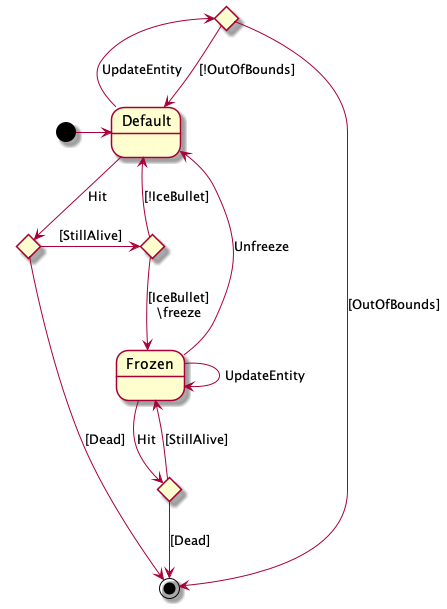
\includegraphics[width=.5\linewidth]{img/state-balloon-actor}
    \caption{Diagramma di stato dell'attore del palloncino.}
    \label{fig:state-balloon-actor}
\end{figure}

\subsubsection{Rounds}
I \textit{round} è rappresentato da una sequenza prestabilita di palloncini che attraversano il percorso e minacciano le
vite a disposizione del giocatore. All'interno di uno stesso \textit{round} possono essere presenti più "ondate" di
palloncini e queste ultime prendono il nome di \texttt{Streak}. L'implementazione più naturale consiste quindi nel
definire un \texttt{Round} come sequenza di \texttt{Streak}, ognuna delle quali è caratterizzata da diversi attributi:
\begin{itemize}
    \item La quantità di palloncini;
    \item Informazioni riguardo al tipo del palloncino: la sua vita ed eventuali potenziamenti;
    \item Il tempo che intercorre tra la generazione di un palloncino e quella del successivo.
\end{itemize}

Per poter definire in modo elegante e conciso un \texttt{Round}, è stata implementata una DSL che quindi permette di
utilizzare la sintassi indicata nel listato \ref{code:rounds} dove \texttt{n}, \texttt{m} e \texttt{l} rappresentano il
numero di palloncini all'interno della \texttt{Streak} corrispondente.
\begin{lstlisting}[label=code:rounds, language=Scala, caption=Esempio di dichiarazione di un \texttt{Round} mediante DSL.]
Round.of(
  Streak(n) :- balloonLife,
  Streak(m) :- (balloonLife & balloonType1 & balloonType2 & ...),
  (Streak(l) :- (balloonLife & balloonType1 & balloonType2 & ...) @@ delay),
)
\end{lstlisting}
Tale sintassi è stata ottenuta sfruttando il pattern \textbf{Pimp My Library} applicato a diverse classi.

Inoltre, è stata resa disponibile anche una sintassi monadica per la definizione del \texttt{Round}. Tale approccio si è
rivelato utile soprattutto per la definizione di \textit{round} più complessi e per garantire maggiore flessiblità: il
precedente approccio obbligava infatti ad inserire tutte le \texttt{Streak} al momento della creazione di un'istanza di
\texttt{Round}, mentre in questo modo è possibile aggiungere \texttt{Streak} in momenti diversi e, quando si è
soddisfatti del risultato, generare il \texttt{Round} complessivo. È possibile apprezzare tale sintassi, realizzata
sfruttando la monade \texttt{IO} della libreria \textit{cats} \cite{cats-effects}, all'interno del listato
\ref{code:roundmonad}.
\begin{lstlisting}[label=code:roundmonad, language=Scala, caption=Esempio di dichiarazione di un \texttt{Round} mediante sintassi monadica.]
(for {
  _ <- define()
  _ <- add(streak1)
  _ <- add(streak2)
} yield ()).built

(for {
  _ <- add(streak3)
} yield ()).built
\end{lstlisting}

\subsubsection{Model Refactor}
La suddivisione della logica del \texttt{Model} nei \textit{manager} è stata resa possibile sfruttando il pattern di
delegazione estremamente comune in \textit{Akka}. In particolare, ad ogni messaggio diretto verso il \texttt{Model} sono
stati assegnati uno o più tipi. L'analisi di un messaggio pertanto produrrà una lista di \texttt{MessageType} che indica
verso quale (o quali) \textit{manager} lo stesso messaggio verrà ridirezionato.

\subsubsection{Positions}
L'implementazione della posizione e della velocità caratterizzanti le entità è stata realizzata mediante un semplice
\textbf{product type} \texttt{Vector2D}. Ciò permette di esprimere le coordinate di un'entità sulla mappa e le
componenti orizzontale e verticale della sua velocità. Sfruttando il pattern \textbf{Pimp My Library} sono stati
aggiunti metodi per la somma tra due \texttt{Vector2D} e per il prodotto con uno scalare in modo che queste operazioni
possano essere effettuate in modo del tutto naturale. Infine, è stato aggiunto un metodo di conversione implicita per
poter creare un \texttt{Vector2D} a partire da una \texttt{Tuple2[Double, Double]} in modo che la definizione risulti
più immediata.

\subsection{Matteo Ragazzini}\label{subsec:matteo-ragazzini}
Il mio compito all'interno del progetto, è stato quello di realizzare il \texttt{TrackLoader} e la relativa pagina
\texttt{SavedTracks}, modellare la gerarchia di \texttt{Entity},  implementare i proiettili e l'attore che
ne definisce il comportamento ed infine gestire l'insermento di animazioni sfruttando il meccanismo delle \textbf{timeline}.
Inoltre, ho collaborato con gli altri membri del team durante la fase di integrazione dei proiettili con torri e palloncini.


\subsubsection{Track Loader}\label{subsec:track-loader}
Uno dei requisiti funzionali espresso dal committente riguardava la possibilità di salvare una traccia di gioco ed in seguito
creare a partire da quest'ultima una nuova partita. Per soddisfare tale requisito ho realizzato la pagina relativa alle
tracce precedentemente salvate \texttt{Saved Tracks} con il relativo controller FXML \texttt{SavedTrackController} e l'attore che gestisce il salvataggio
e il caricamento di tali tracce, il \texttt{TrackLoader}.

Il \texttt{TrackLoader} ha tre compiti fondamentali:
\begin{itemize}
    \item restituire al \texttt{SavedTrackController} tutte le tracce precendentemente salvate quando l'utente
        dal main menù accede alla pagina \texttt{Saved Tracks};
    \item fornire al \texttt{Model} la traccia selezionata dall'utente nella pagina \texttt{Saved Tracks}.
          In questo modo il \texttt{Model} può procedere alla creazione di una nuova partita con la suddetta traccia;
    \item salvare una nuova traccia, realizzando inoltre tramite lo \texttt{ScreenShooter} un screenshot di quest'ultima,
    in modo da fornire all'utente un riscontro visivo della traccia salvata all'interno della pagina \texttt{Saved Tracks}.
\end{itemize}

Per ottenere persistenza delle tracce salvate il \texttt{TrackLoader} fa uso di un \texttt{FileCoder}, componente realizzato
da Tommaso Mandoloni per la serializzazione e deserializzazione di tracce su file.

L'interazione fra \texttt{TrackLoader} e \texttt{FileCoder} è riportata nel diagramma di sequenza in figura \ref{fig:sequence-track-loader}.


\begin{figure}[H]
    \centering
    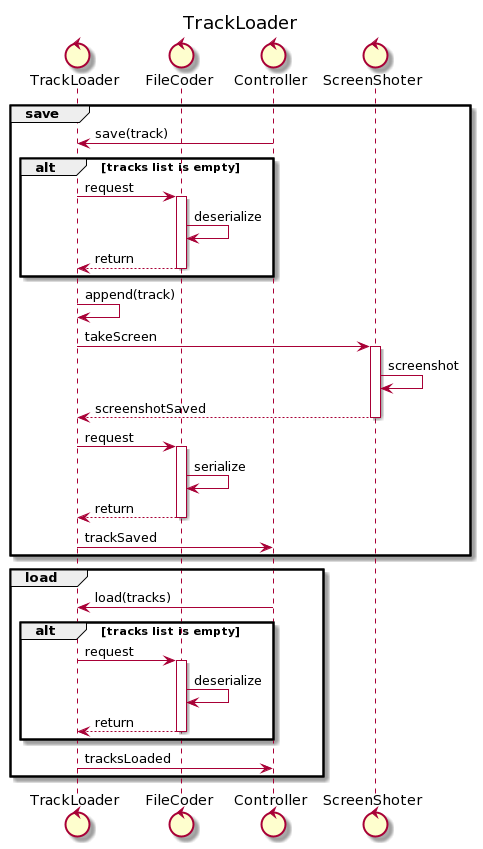
\includegraphics[width=.57\linewidth]{img/sequence-track-loader}
    \caption{Diagramma di sequenza dell'interazione fra \texttt{TrackLoader}, \texttt{FileCoder} e \texttt{Controller}.}
    \label{fig:sequence-track-loader}
\end{figure}



\subsubsection{Proiettili}
I proiettili rappresentano all'interno del gioco il componente di più basso livello, che viene sparato dalle torri
per infliggere danni ai palloncini. Il \texttt{trait Bullet} è quindi rappresentato dall'estensione del
\texttt{trait Entity} a cui è stata aggiunta l'abilità di movimento (\texttt{Movement Ability})

In fase di definizione dei requisiti sono stati individuati tre tipi diversi di proiettili: freccetta, bomba e palla di neve.
Questi ultimi presentano un comportamento comune: possiedono una posizione, una velocità, una dimensione ed un danno, ma
la bomba e la palla di neve in quanto proiettili esplosivi devono infliggere danni all'interno di un'area; inoltre
la palla di neve possiede anche l'abilità di congelamento che, oltre ad infliggere danni, congela i palloncini colpiti
lungo il tracciato.

Per l'implementazione di \texttt{Dart}, \texttt{CannonbBall} e \texttt{IceBall} si è quindi partiti col definire una case class
di base, la \texttt{BasicBullet} che definisce i tratti comuni fra le tre entità. Successivamente si è deciso di realizzare
le entità di più alto livello, come wrapper di una \texttt{BasicBullet}, alla quale vengono aggiunte delle proprietà.

Per esempio, grazie alla buona gerarchia di carattereristiche definite in \texttt{Entity} è stato possibile riutilizzare
il trait \texttt{SightRange} (inizialmente pensato per le torri) per dotare il trait \texttt{Explosion} dell'abilità di
individuare la collisione con altre entità all'interno di un certo sightRange e quindi "esplodere". Tale trait è stato
successivamente esteso da \texttt{Fire} e \texttt{Ice}, rispettivamente rappresentati esplosioni di fuoco e di ghiaccio.

A questo punto grazie ai \textbf{mixin} è stato possibile definire ad esempio una \texttt{CannonbBall} come
\texttt{Bullet} \textbf{with} Fire.

Volendo seguire un approccio puramente funzionale i metodi di aggiornamento di un bullet devono crearne uno nuovo
con i valori aggiornati. Questo comportamento è comune a tutti i bullet, ma l'aggiornamento
di ognuno questi deve tornare il tipo di bullet corretto, per questo avrei dovuto implementare tali
metodi all'interno di ogni tipo di proiettile. Per evitare un'inutile ripetizione
di codice ho realizzato un metodo instance, di cui ogni sottoentità ne effettua l'override, per restituire l'istanza
corretta del Bullet da ricreare. I metodi di aggiornamento sono stati quindi posti all'interno di BasicBullet e questi
richiamano il metodo \textbf{instance()}.

Infine è stato realizzato un oggetto \textbf{Shooting} con metodo \textbf{from} che permette passata una \textbf{[Tower[Bullet]]}
di sparare un nuovo proiettile del tipo corrispondente alla tower, con il giusto danno, posizione e direzione.

\begin{lstlisting}[label=code:bullet, language=Scala, caption=Implementazione dei bullet con focus sulla CannonBall]

trait Bullet extends Entity with MovementAbility {
    type Boundary = (Double, Double)

    override def position: Vector2D = bullet.position
    override def speed: Vector2D = bullet.speed
    override def boundary: Boundary = bullet.boundary

    override def in(pos: Vector2D): Bullet = instance(
    BasicBullet(this.damage, pos, this.speed, this.boundary)
    )

    override def at(velocity: Vector2D): Bullet = instance(
    BasicBullet(this.damage, this.position, velocity, this.boundary)
    )

    def damage: Double = bullet.damage
    def hurt(d: Double): Bullet = instance(BasicBullet(d, this.position, this.speed, this.boundary))

    def bullet: Bullet
    def instance(bullet: Bullet): Bullet
}

case class BasicBullet(
    override val damage: Double = bulletDefaultDamage,
    override val position: Vector2D = defaultPosition,
    override val speed: Vector2D = bulletDefaultSpeed,
    override val boundary: (Double, Double) = bulletDefaultBoundary)
    extends Bullet {
    override def instance(b: Bullet): Bullet = b

    override def bullet: Bullet = this
}

trait Explosion extends Bullet with SightAbility

trait Fire extends Explosion

/** Adds to the [[Bullet]] the exploding ability */
case class CannonBall(
   override val bullet: Bullet = BasicBullet(),
   override val sightRange: Double = bulletDefaultSightRange)
   extends Bullet
   with Fire {
   override def instance(b: Bullet): Bullet = CannonBall(b, sightRange)

   override def sight(radius: Double): Explosion = CannonBall(bullet, radius)
}
\end{lstlisting}

Avendo adottato una architettura ad attori, ogni proiettile, in fase di creazione, viene associato ad un attore che ne definisce
il comportamento, mostrato in figura \ref{fig:sequence-bullet-actor}. Tale attore presenta due \texttt{Behaviour}: \
texttt{default} ed \texttt{exploding}.
Quando l'attore è nel behaviour di \texttt{default} aggiorna la posizione del bullet, verifica che questo non esca dal campo visivo e
cosa più importante controlla che non sussistano collisioni con dei palloncini, caso nel quale, l'attore cambia comportamento
passando ad \texttt{explosion}.
In \texttt{explosion} l'attore notifica il model con la lista di palloncini colpiti, in caso il bullet sia di tipo
\texttt{Explosion} ne avvia l'animazione ed infine notifica il model chiedendo di rimuovere il bullet dalla lista di entità
in gioco.


\begin{figure}[H]
    \centering
    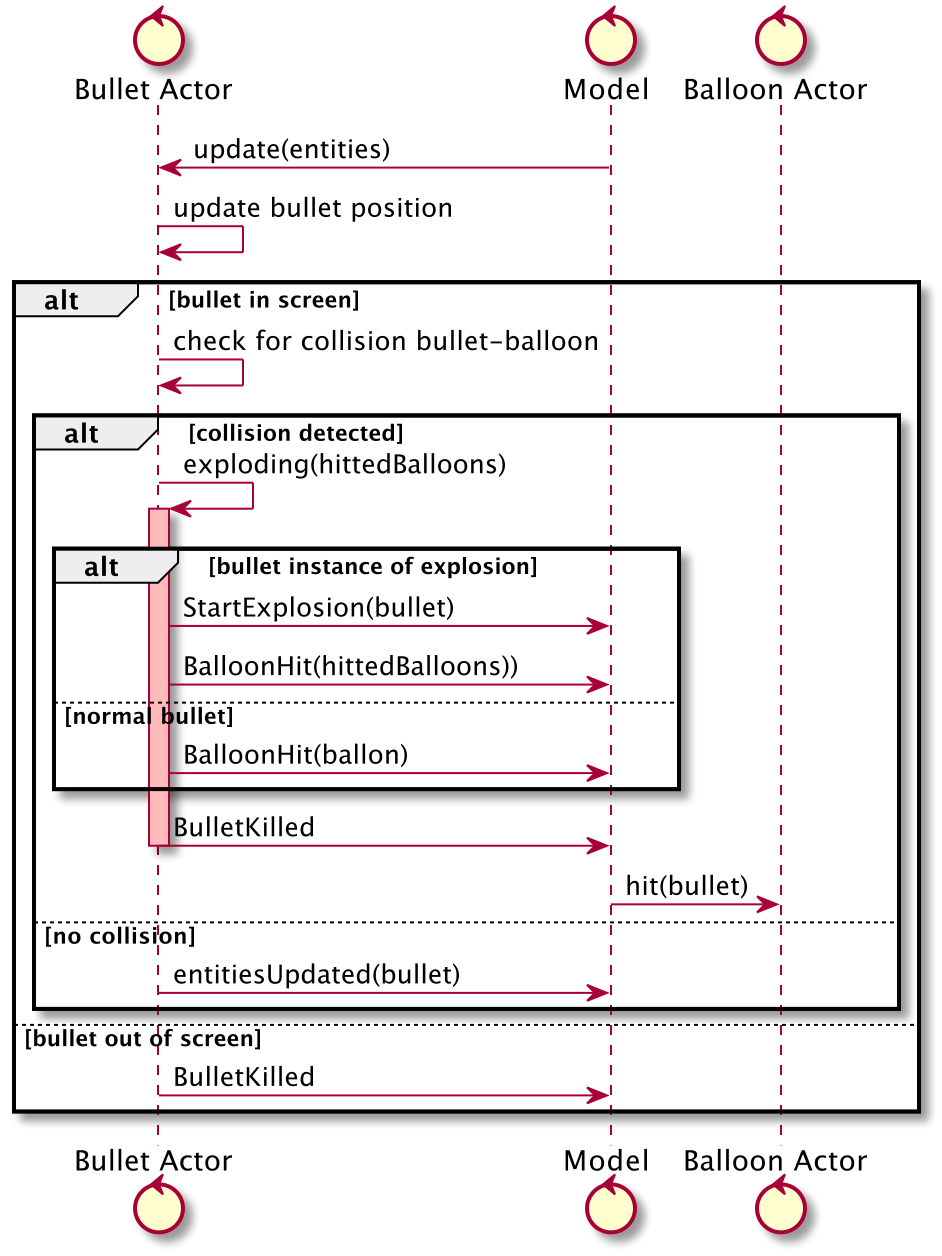
\includegraphics[width=.7\linewidth]{img/sequence-bullet-actor}
    \caption{Diagramma di sequenza delle interazioni del \texttt{bulletActor}.}
    \label{fig:sequence-bullet-actor}
\end{figure}

\subsection{Simone Romagnoli}
Fungendo da \textit{product owner}, le porzioni di progetto di cui mi sono occupato sono molteplici: oltre ad aver
proposto il design dell'architettura complessiva, ho partecipato all'implementazione di svariate parti del sistema e, a
volte, ho rivalutato l'effettiva scrittura di alcune funzionalità. Di seguito, descrivo le parti significative del mio
lavoro, focalizzandomi sugli aspetti implementativi importanti per la totalità del progetto.

\subsubsection{Tracce di gioco}
La mappa del gioco è descritta da una griglia invisibile composta da celle: le tracce non sono altro
che una sequenza ordinata di celle adiacenti, a partire dal bordo sinistro dello schermo, e a terminare in quello
destro. Per elaborare il tracciato che i palloncini seguono durante la partita, ho deciso di sfruttare la programmazione
logica, e, nello specifico, la libreria \texttt{it.unibo.alice.tuprolog} \cite{tp}. In ausilio alla interazione
\textit{Scala-Prolog}, è stato implementato un motore specifico \ref{code:prolog-engine} che risolve le query in input,
trovando una traccia con fattori di casualità.

\begin{lstlisting}[label=code:prolog-engine, language=Scala, caption=Motore TuProlog]
/** A Prolog engine that solves queries. */
case class PrologEngine(theory: Theory) extends Engine {
  val engine: Prolog = new Prolog
  engine.setTheory(theory)

  override def solve: Term => LazyList[SolveInfo] = term =>
    LazyList.continually(engine solve term)

}
\end{lstlisting}

Le query vengono formulate prendendo in input tre parametri:
\begin{itemize}
    \item una cella d'inizio;
    \item una cella di fine;
    \item la difficoltà di gioco.
\end{itemize}

Sulla base di questi, viene trovata una soluzione con la teoria sviluppata: il metodo tradizionale per trovare una
traccia, sarebbe quello di calcolare tutti i possibili percorsi dalla cella d'inizio a quella di fine e sceglierne uno
casualmente; tuttavia, questo approccio è risultato essere troppo oneroso, già a partire da griglie di dimensione
$5 \times 5$. Il metodo utilizzato per individuare una traccia soddisfacente, è stato quello di disegnarne una
introducendo fattori di casualità nel processo di scelta delle celle, ad esempio, implicando un cambiamento di direzione
sempre più probabile con l'aumentare di celle consecutive aventi lo stesso orientamento. Anche la difficoltà di gioco
è un fattore determinante: la traccia, infatti, non torna mai verso la cella d'inizio quando la difficoltà è difficile,
in modo da accorciare la traccia e facilitare i palloncini, mentre, in modalità facile, è più probabile ottenere una
traccia più lunga.

\subsubsection{Abilità di TrackFollowing}
Per muovere i palloncini sulla traccia, sarebbe corretto rispettare la gerarchia di entità mostrata nella sezione
\ref{sec:detailed-design}, in particolare, senza modificare l'interfaccia \texttt{MovementAbility}, bensì aggiungendo una
funzionalità ad essa. Quindi è stato pensato un meccanismo che associa una posizione lineare al palloncino sulla
traccia bidimensionale: il \texttt{TrackFollowing}. L'abilità di movimento viene sovrascritta in base alla posizione
lineare nella traccia. Nello specifico, la posizione lineare è stata pensata come un \texttt{Double} la cui parte
intera rappresenta l'indice della cella occupata dal palloncino nella traccia, mentre la parte decimale indica la
percentuale attraversata della cella stessa. Inoltre, la posizione lineare rende i palloncini effettivamente confrontabili,
riuscendo a valutare quale di questi sia il più pericoloso poiché più vicino alla fine del percorso;
infatti, l'interfaccia \texttt{Track Following} estende anche \texttt{Comparable}. Quest'ultima proprietà viene sfruttata
anche a livello di renderizzazione disegnando i palloncini ordinati.

\subsubsection{Rendering DSL}
Vista la complessità dei \textit{controller fxml}, è stato implementato un \textit{domain-specific language} che
semplifica la creazione di elementi grafici con una sintassi espressiva e sintetica. A tale scopo, è stato creato
l'oggetto \texttt{Rendering} che fornisce un metodo per disegnare oggetti di diverso tipo: per farlo, è stato
implementato un generico \texttt{Drawer} che, utilizzando il pattern \textit{type-class}, permette di
disegnare svariate entità. Il listato \ref{code:rendering} mostra gli strumenti utilizzati per tale procedura.

\begin{lstlisting}[label=code:rendering, language=Scala, caption=Implementazione della \textit{dsl} \texttt{Rendering}]
/** Simulates a DSL for rendering logic entities. */
object Rendering {

  /** Draws a generic element with an implicit drawer. */
  def a[T](element: T)(implicit drawer: Drawer[T]): Renderable = drawer.draw(element)

  /** Contains all the implicit drawers that allow to render graphical elements. */
  object Drawers {

    /** Allows to turn a generic element into a [[Renderable]]. */
    trait Drawer[-T] {
      def draw(elem: T): Renderable
    }

    implicit val gridDrawer = ...
    implicit val trackDrawer = ...
    implicit val entityDrawer = ...
  }
}
\end{lstlisting}

In questo modo, viene semplificata la creazione di elementi grafici comuni in più \textit{controller fxml}, come, ad
esempio, le torri disegnate sia nel \texttt{GameController} sia nel \texttt{GameMenuController}. L'interfaccia
\texttt{Renderable} è semplicemente un contenitore di \texttt{Shape} di \textit{ScalaFX}. Inoltre, si sottolinea che il
\texttt{Drawer} deve essere necessariamente controvariante per via della gerarchia di entità da renderizzare: infatti,
ha senso che un \texttt{Drawer[Entity]} sappia disegnare una torre, mentre un \texttt{Drawer[Tower]} non sappia
disegnare una entità, rendendo, di fatto, il primo sottotipo del secondo. Nel listato \ref{code:view-draw} si mostrano
due diverse applicazioni del \textit{domain-specific language} appena descritto.

\begin{lstlisting}[label=code:view-draw, language=Scala, caption=Applicazione della \textit{dsl} \texttt{Rendering}]
/** Renders a track into the proper pane. */
override def draw(track: Track): Unit = Platform runLater {
    Rendering a track into trackPane.children
    trackChoiceController.show()
}

/** Renders a list of entities into the proper pane. */
override def draw(entities: List[Entity]): Unit = Platform runLater {
    entitiesPane.children.clear()
    entities foreach (entity => Rendering a entity into entitiesPane.children)
}
\end{lstlisting}


